\documentclass[12pt,a4paper]{article}
\usepackage[utf8]{inputenc}
\usepackage[spanish]{babel}
\usepackage{amsmath}
\usepackage{amsfonts}
\usepackage{amssymb}
\usepackage{graphicx}
\usepackage[left=2cm,right=2cm,top=2cm,bottom=2cm]{geometry}
\author{APLICACIONES DE MANIPULADORES PARALELOS.\\Enciso Guerrero Benjamin Salvador\\
Carlos Enrrique Moran Garabito\\
Cinematica De Robots }
\title{UNIVERSIDAD POLITECNICA DE LA ZONA METROPOLITANA DE GUADALAJARA.}
\begin{document}
\maketitle

\includegraphics[scale=1.8]{upzmgg.jpg} 
\newpage
APLICACIONES DE MANIPULADORES PARALELOS.
\\\\
Hoy en día los robots son parte fundamental de nuestra industria, facilitando la ejecución de múltiples tareas, aumentando la precisión del producto final y disminuyendo tiempos de ejecución. Además, son muchos otros los ámbitos en los que los sistemas robóticos modernos colaboran, como pueden ser el sector aeroespacial, diversas aplicaciones médicas, industria de los videojuegos, etc. 
\\\\
En particular, los denominados manipuladores paralelos han ido adquiriendo en los últimos años una notable relevancia, existiendo numerosas líneas de investigación y proyectos asociados al estudio y desarrollo de este tipo de robots. Sin embargo, en ocasiones, no siempre existe una comunicación bilateral entre industria e investigación, o incluso entre las propias ramas de investigación existentes, de forma que se crea un cierto desconocimiento acerca de los trabajos realizados, los que están en proceso de ejecución y las posibles líneas de trabajo futuras. 
\\\\
Por ello, cuando un determinado ámbito del conocimiento alcanza un cierto grado de madurez, conviene reflejar su actual estado de la técnica. 
\\\\
APLICACIONES.
\\\\
Se proponen aplicaciones en las que pueden ser utilizados dichos manipuladores haciendo uso de sus configuraciones de insensitividad positiva para el posicionamiento de piezas o herramientas en procesos de fabricación.
\\\\
Aplicaciones de vuelo(CAE)
\\
\begin{center}
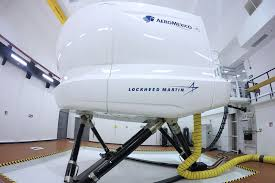
\includegraphics[scale=0.7]{1.jpg}
\end{center}
\begin{center}
Imagen 1 simulacion de vuelo
\end{center}

Maquinado de piezas (Ingersoll)
\\
\begin{center}
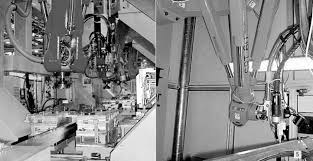
\includegraphics[scale=0.7]{2.jpg} 
\end{center}
\begin{center}
Imagen 2 maquinado de piezas
\end{center}

\newpage

Transporte de objetos (Fanuc)
\\
\begin{center}
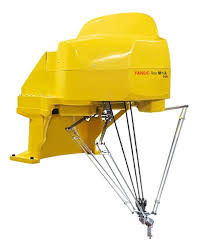
\includegraphics[scale=1]{03.jpg} 
\end{center}
\begin{center}
Imagen 3 Robot (FANUC)
\end{center}

Posicionamiento de precisión (PI)
\begin{center}
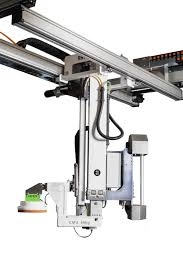
\includegraphics[scale=1]{3.jpg} 
\end{center}
\begin{center}
Imagen 4 Robot cartesiano.
\end{center}
\newpage
Dispositivos Hapticos 
\\
\begin{center}
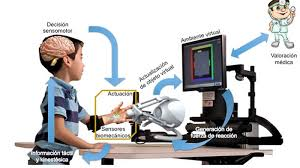
\includegraphics[scale=1.2]{5.jpg} 
\end{center}
\begin{center}
Imagen 5 Dispositivo Haptico
\end{center}

Robots submarinos 
\begin{center}
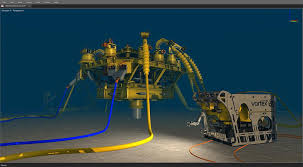
\includegraphics[scale=1.3]{6.jpg} 
\end{center}
\begin{center}
Imagen 6 Robot Submarino.
\end{center}




\end{document}